\usepackage{amsmath,amssymb, amsthm}             % AMS Math
\usepackage[T1]{fontenc}
\usepackage[utf8x]{inputenc}
\usepackage{babel}
\usepackage{datetime}

\usepackage{silence}

\WarningFilter{minitoc(hints)}{W0023}
\WarningFilter{minitoc(hints)}{W0028}
\WarningFilter{minitoc(hints)}{W0030}

\usepackage{lmodern}
\usepackage{tabularx}
%\usepackage{tabular}
\usepackage{multirow}
\usepackage{xspace}

\usepackage{subfig}
\usepackage[inline]{enumitem}

\usepackage{hhline}
\usepackage[left=1.5in,right=1.3in,top=1.1in,bottom=1.1in,includefoot,includehead,headheight=13.6pt]{geometry}
\renewcommand{\baselinestretch}{1.05}

% Table of contents for each chapter

\usepackage[nottoc, notlof, notlot]{tocbibind}
\usepackage{minitoc}
\setcounter{minitocdepth}{2}
\mtcindent=15pt
% Use \minitoc where to put a table of contents

\usepackage{aecompl}

% Glossary / list of abbreviations

\usepackage[intoc]{nomencl}
\iftoggle{ThesisInEnglish}{%
\renewcommand{\nomname}{Glossary}
}{ %
\renewcommand{\nomname}{Liste des Abréviations}
}

\usepackage{etoolbox}
\renewcommand\nomgroup[1]{%
  \item[\bfseries
  \ifstrequal{#1}{A}{Number Sets}{%
  \ifstrequal{#1}{G}{Agents Beliefs and Action Models}{%
  \ifstrequal{#1}{N}{Navigation}{%
  \ifstrequal{#1}{O}{Ontology}{%
  \ifstrequal{#1}{R}{Referring Expression Generation}{%
  \ifstrequal{#1}{Z}{Controllable and Uncontrollable Agents Task Planning}{}}}}}}%
]}

\makenomenclature



% My pdf code

\usepackage{ifpdf}

\ifpdf
  \usepackage[pdftex]{graphicx}
  \DeclareGraphicsExtensions{.jpg}
  \usepackage[pagebackref,hyperindex=true]{hyperref}
  \usepackage{tikz}
  \usetikzlibrary{arrows,shapes,calc}
\else
  \usepackage{graphicx}
  \DeclareGraphicsExtensions{.ps,.eps}
  \usepackage[dvipdfm,pagebackref,hyperindex=true]{hyperref}
\fi

\graphicspath{{.}{images/}}

%% nicer backref links. NOTE: The flag ThesisInEnglish is used to define the
% language in the back references. Read more about it in These.tex

\iftoggle{ThesisInEnglish}{%
\renewcommand*{\backref}[1]{}
\renewcommand*{\backrefalt}[4]{%
\ifcase #1 %
(Not cited.)%
\or
(Cited in page~#2.)%
\else
(Cited in pages~#2.)%
\fi}
\renewcommand*{\backrefsep}{, }
\renewcommand*{\backreftwosep}{ and~}
\renewcommand*{\backreflastsep}{ and~}
}{%
\renewcommand*{\backref}[1]{}
\renewcommand*{\backrefalt}[4]{%
\ifcase #1 %
(Non cité.)%
\or
(Cité en page~#2.)%
\else
(Cité en pages~#2.)%
\fi}
\renewcommand*{\backrefsep}{, }
\renewcommand*{\backreftwosep}{ et~}
\renewcommand*{\backreflastsep}{ et~}
}

% Links in pdf
\usepackage{color}
\definecolor{linkcol}{rgb}{0,0,0.4} 
\definecolor{citecol}{rgb}{0.5,0,0} 
\definecolor{linkcol}{rgb}{0,0,0} 
\definecolor{citecol}{rgb}{0,0,0}
% Change this to change the informations included in the pdf file

\hypersetup
{
bookmarksopen=true,
pdftitle="Endowing the robot with the abilities to control and evaluate its contribution to a human-robot joint action",
pdfauthor="Amandine MAYIMA", %auteur du document
pdfsubject="Thèse", %sujet du document
%pdftoolbar=false, %barre d'outils non visible
pdfmenubar=true, %barre de menu visible
pdfhighlight=/O, %effet d'un clic sur un lien hypertexte
colorlinks=true, %couleurs sur les liens hypertextes
pdfpagemode=None, %aucun mode de page
pdfpagelayout=SinglePage, %ouverture en simple page
pdffitwindow=true, %pages ouvertes entierement dans toute la fenetre
linkcolor=linkcol, %couleur des liens hypertextes internes
citecolor=citecol, %couleur des liens pour les citations
urlcolor=linkcol %couleur des liens pour les url
}

% definitions.
% -------------------

\setcounter{secnumdepth}{3}
\setcounter{tocdepth}{2}

% Some useful commands and shortcut for maths:  partial derivative and stuff

\newcommand{\pd}[2]{\frac{\partial #1}{\partial #2}}
\def\abs{\operatorname{abs}}
\def\argmax{\operatornamewithlimits{arg\,max}}
\def\argmin{\operatornamewithlimits{arg\,min}}
\def\diag{\operatorname{Diag}}
\newcommand{\eqRef}[1]{(\ref{#1})}

\usepackage{rotating}                    % Sideways of figures & tables
%\usepackage{bibunits}
%\usepackage[sectionbib]{chapterbib}          % Cross-reference package (Natural BiB)
\usepackage{natbib}                  % Put References at the end of each chapter
                                         % Do not put 'sectionbib' option here.
                                         % Sectionbib option in 'natbib' will do.
\usepackage{fancyhdr}                    % Fancy Header and Footer

% \usepackage{txfonts}                     % Public Times New Roman text & math font
  
%%% Fancy Header %%%%%%%%%%%%%%%%%%%%%%%%%%%%%%%%%%%%%%%%%%%%%%%%%%%%%%%%%%%%%%%%%%
% Fancy Header Style Options

\pagestyle{fancy}                       % Sets fancy header and footer
\fancyfoot{}                            % Delete current footer settings

%\renewcommand{\chaptermark}[1]{         % Lower Case Chapter marker style
%  \markboth{\chaptername\ \thechapter.\ #1}}{}} %

%\renewcommand{\sectionmark}[1]{         % Lower case Section marker style
%  \markright{\thesection.\ #1}}         %

\fancyhead[LE,RO]{\bfseries\thepage}    % Page number (boldface) in left on even
% pages and right on odd pages
\fancyhead[RE]{\bfseries\nouppercase{\leftmark}}      % Chapter in the right on even pages
\fancyhead[LO]{\bfseries\nouppercase{\rightmark}}     % Section in the left on odd pages

\let\headruleORIG\headrule
\renewcommand{\headrule}{\color{black} \headruleORIG}
\renewcommand{\headrulewidth}{1.0pt}
\usepackage{colortbl}
\arrayrulecolor{black}

\fancypagestyle{plain}{
  \fancyhead{}
  \fancyfoot{}
  \renewcommand{\headrulewidth}{0pt}
}

%\usepackage{MyAlgorithm}
%\usepackage[noend]{MyAlgorithmic}
\usepackage{algorithm}
\usepackage[noend]{algpseudocode}
\usepackage{comment}
\usepackage[ED=MITT-InfoTel, Ets=INSA]{tlsflyleaf}
%%% Clear Header %%%%%%%%%%%%%%%%%%%%%%%%%%%%%%%%%%%%%%%%%%%%%%%%%%%%%%%%%%%%%%%%%%
% Clear Header Style on the Last Empty Odd pages
\makeatletter

\def\cleardoublepage{\clearpage\if@twoside \ifodd\c@page\else%
  \hbox{}%
  \thispagestyle{empty}%              % Empty header styles
  \newpage%
  \if@twocolumn\hbox{}\newpage\fi\fi\fi}

\newcommand*{\algrule}[1][\algorithmicindent]{%
	\makebox[#1][l]{%
		\hspace*{.2em}% <------------- This is where the rule starts from
		\vrule height .75\baselineskip depth .25\baselineskip
	}
}

%%% to have lines in algorithm, from stackexchange
\newcount\ALG@printindent@tempcnta
\def\ALG@printindent{%
	\ifnum \theALG@nested>0% is there anything to print
	\ifx\ALG@text\ALG@x@notext% is this an end group without any text?
	% do nothing
	\else
	\unskip
	% draw a rule for each indent level
	\ALG@printindent@tempcnta=1
	\loop
	\algrule[\csname ALG@ind@\the\ALG@printindent@tempcnta\endcsname]%
	\advance \ALG@printindent@tempcnta 1
	\ifnum \ALG@printindent@tempcnta<\numexpr\theALG@nested+1\relax
	\repeat
	\fi
	\fi
}
% the following line injects our new indent handling code in place of the default spacing
\patchcmd{\ALG@doentity}{\noindent\hskip\ALG@tlm}{\ALG@printindent}{}{\errmessage{failed to patch}}
\patchcmd{\ALG@doentity}{\item[]\nointerlineskip}{}{}{} % no spurious vertical space
% end vertical rule patch for algorithmicx

%modify \@endpart so it doesn't produce a blank page
\renewcommand{\@endpart}{\vfil\newpage}

\makeatother
 
%%%%%%%%%%%%%%%%%%%%%%%%%%%%%%%%%%%%%%%%%%%%%%%%%%%%%%%%%%%%%%%%%%%%%%%%%%%%%%% 
% Prints your review date and 'Draft Version' (From Josullvn, CS, CMU)
\newcommand{\reviewtimetoday}[2]{\special{!userdict begin
    /bop-hook{gsave 20 710 translate 45 rotate 0.8 setgray
      /Times-Roman findfont 12 scalefont setfont 0 0   moveto (#1) show
      0 -12 moveto (#2) show grestore}def end}}
% You can turn on or off this option.
% \reviewtimetoday{\today}{Draft Version}
%%%%%%%%%%%%%%%%%%%%%%%%%%%%%%%%%%%%%%%%%%%%%%%%%%%%%%%%%%%%%%%%%%%%%%%%%%%%%%% 

\newenvironment{maxime}[1]
{
\vspace*{0cm}
\hfill
\begin{minipage}{0.5\textwidth}%
%\rule[0.5ex]{\textwidth}{0.1mm}\\%
\hrulefill $\:$ {\bf #1}\\
%\vspace*{-0.25cm}
\it 
}%
{%

\hrulefill
\vspace*{0.5cm}%
\end{minipage}
}

\let\minitocORIG\minitoc
\renewcommand{\minitoc}{\minitocORIG \vspace{1.5em}}

\usepackage{multirow}
%\usepackage{slashbox}

\newenvironment{bulletList}%
{ \begin{list}%
	{\tiny$\bullet$}%
	{\setlength{\labelwidth}{25pt}%
	 \setlength{\leftmargin}{30pt}%
	 \setlength{\itemsep}{-0.5em}}}%
{ \end{list} }

\newenvironment{enumList}%
{ \begin{enumerate}[noitemsep]
		\setlength{\leftmargin}{30pt}}%
	{ \end{enumerate} }

\newenvironment{inlineEnumerate}
{\begin{enumerate*} [label={(\arabic*)}] }
{\end{enumerate*}}

\theoremstyle{definition}
\newtheorem{definition}{Definition}
\renewcommand{\epsilon}{\varepsilon}

% centered page environment

\newenvironment{vcenterpage}
{\newpage\vspace*{\fill}\thispagestyle{empty}\renewcommand{\headrulewidth}{0pt}}
{\vspace*{\fill}}

\newenvironment{asl}{\ttfamily\begin{tabbing}~~~\=$\leftarrow$ \= ~~~ \=
		\kill}{\end{tabbing}}

\usepackage{tablefootnote}

\theoremstyle{plain}
\newtheorem{constraint}{Constraint}[section]

\algnewcommand\algorithmicforeach{\textbf{for each}}
\algnewcommand\algorithmicin{\textbf{in}}
\algdef{S}[FOR]{ForEach}[2]{\algorithmicforeach\ #1\ \algorithmicin\ #2\ \algorithmicdo}

\algnewcommand\algorithmicforkxor{\textbf{do fork-join-xor}}
\algnewcommand\algorithmicendforkxor{\textbf{end fork-join-xor}}
\algdef{SE}{ForkXor}{EndForkXor}{\algorithmicforkxor}{\algorithmicendforkxor}


\usepackage{listings}
\lstset{
	frame=single,
	captionpos=b,
	breaklines=true,
	basicstyle=\ttfamily,
	numberstyle=\color{black},
	tabsize=2,
	mathescape=true,
	literate=%
		{â}{{\^a}}1
}

\lstdefinestyle{inline}{
	frame=none,
	aboveskip=\smallskipamount,
	belowskip=\smallskipamount,
}

\lstdefinestyle{OwlTurtle}{
	language=C,
	tabsize=4,
	basicstyle=\scriptsize\ttfamily,
	keywordstyle=\bfseries\color{darkgray},
	morekeywords={rdf:type, rdfs:domain, rdfs:subPropertyOf, rdfs:range, :hasSubtask, :DecompositionUsedBy, rdfs:subClassOf, :hasDecomposition, owl:inverseOf, htn_actions:hasEffect, rdfs:label},
	alsoletter=:
}

\lstdefinestyle{aslDef}{
	frame=none,
%	breaklines=false,
	%xleftmargin=.1\textwidth, xrightmargin=.1\textwidth
}

\fancypagestyle{example}{%
	\fancyhead[LE]{\bfseries\thepage
\includegraphics[scale=0.20]{figures/chapter2/task_goal.pdf}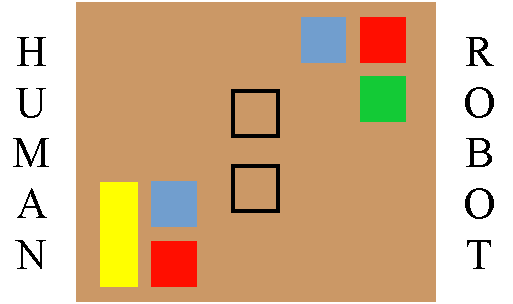
\includegraphics[scale=0.18]{figures/chapter2/task_setup_mini.pdf}}   
	\fancyhead[RO]{
\includegraphics[scale=0.20]{figures/chapter2/task_goal.pdf}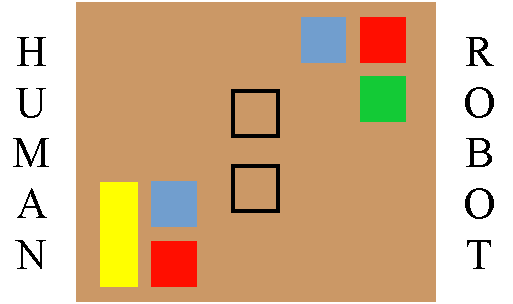
\includegraphics[scale=0.18]{figures/chapter2/task_setup_mini.pdf}\bfseries\thepage}  
	\fancyhead[RE]{\bfseries\nouppercase{\leftmark}}      % Chapter in the right on even pages
	\fancyhead[LO]{\bfseries\nouppercase{\rightmark}}     % Section in the left on odd pages
}%


\newenvironment{partintro}
{\vspace*{\fill}
	\thispagestyle{plain}
	\section*{\centering Introduction to part \thepart}
	\begin{quotation}}
	{\end{quotation}\vspace*{\fill}\newpage}
\newcommand{\nopartintro}{%
	\vspace*{\fill}
	\thispagestyle{empty}
	\newpage
}

\usepackage{pdfpages}
\usepackage{makecell}
\usepackage{pdflscape} 
\usepackage{mathtools}
\usepackage[section]{placeins}
\usepackage{afterpage}
\usepackage{bookmark}

%%%%%%%% my commands
\newcommand{\etal}{\textit{et al}.}
\newcommand{\ie}{\textit{i.e.}, }
\newcommand{\eg}{\textit{e.g.}, }
\newcommand{\fact}[3]{\mbox{\textit{#1}(#2, #3)}}
\newcommand{\circledtext}[1]{\raisebox{.5pt}{\textcircled{\raisebox{-.9pt} {#1}}}}
\newcommand{\sparql}{\textsc{SPARQL}}

\newcommand{\algConst}[1]{${\scriptscriptstyle #1}$}
\newcommand{\algNormTextSub}[2]{$\text{#1}_{#2}$}

\newcommand{\aslnumber}[1]{$#1$}
\newcommand{\aslstring}[1]{\textsf{#1}}
\newcommand{\aslvar}[1]{\textcolor{purple}{\textit{#1}}}
\newcommand{\asllabel}[1]{\textbf{#1}}
\newcommand{\annotation}[1]{{\footnotesize #1}}
\newcommand{\rulebody}[1]{\mbox{\hspace{.05\linewidth}}\begin{minipage}[t]{0.9\linewidth}#1.\end{minipage}}
\newcommand{\context}[1]{\begin{minipage}[t]{0.9\linewidth}#1\end{minipage}}
\newcommand{\planbody}[1]{\begin{minipage}[t]{0.9\linewidth}#1.\end{minipage}}
\newcommand{\Jason}[0]{\textbf{\textit{Jason}}}
\newcommand{\sn}{\mbox{\large\textbf{\texttt{\textasciitilde}}}}
